
\question آقا
طرفای صفحه ۸ اسلاید ۴ یه دیاگرامی بود که خیلی شیک اسکیپ کردید. چی میگفت
حالا؟ داشت نشون می‌داد که اگر وسط کار
CPU
عزیز یه وقفه ایجاد بشه، روند انجام کارها به چه صورت پیش می‌رِد!
چون حوصله باز کردن اسلاید‌ها رو ندارید عکسشو میذاریم اینجا:
\begin{center}
    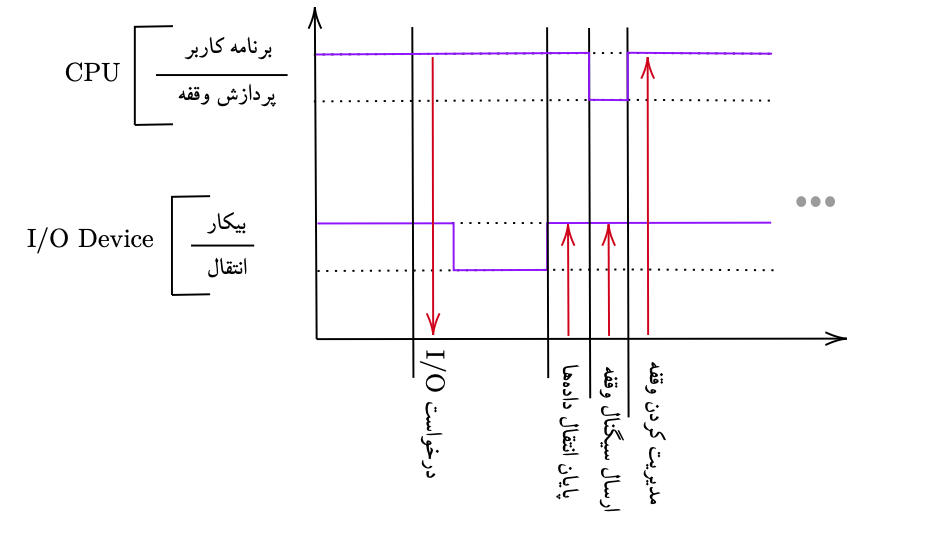
\includegraphics[scale=0.9]{images/diagram.png}
\end{center}

اول خوب تحلیلش کنید و بعد سناریوی زیر رو بخونید:
\begin{enumerate}
    \item یک فرایند کاربر که روی CPU در حال اجراست، یک درخواست ورودی/خروجی (I/O) به دیسک ارسال می‌کند. به جای اینکه CPU هر انتقال داده را با وقفه‌ها مدیریت کند، از
          \lr{DMA (Direct Memory Access)}
          استفاده می‌کند.
    \item وقتی درخواست I/O داده می‌شود، CPU کنترلر DMA را برنامه‌ریزی کرده و سپس اجرای فرایند کاربر را ادامه می‌دهد.
    \item کنترلر DMA انتقال داده‌ها بین حافظه و دستگاه ورودی/خروجی را مستقیماً برعهده می‌گیرد، در حالی که CPU آزاد است تا دستورهای کاربر را اجرا کند.
    \item وقتی انتقال کامل شد، کنترلر DMA یک وقفه به CPU می‌فرستد. CPU به‌طور کوتاه وقفه را رسیدگی کرده و سپس اجرای فرایند کاربر را از سر می‌گیرد.
\end{enumerate}

\begin{parts}
    \pagebreak
    \part[15] حالا با توجه به سناریوی بالا، دیاگرام پایین رو کامل کنید.

    % \vspace{1cm}
    \begin{center}
        \scalebox{0.8}{ 
\tikzset{every picture/.style={line width=0.75pt}} %set default line width to 0.75pt        

\begin{tikzpicture}[x=0.75pt,y=0.75pt,yscale=-1,xscale=1]
%uncomment if require: \path (0,455); %set diagram left start at 0, and has height of 455

%Straight Lines [id:da23411427234450732] 
\draw    (130,20.96) -- (130,130.96) ;
%Straight Lines [id:da2889349755532342] 
\draw    (197,50.96) -- (130,50.96) ;
%Straight Lines [id:da21977095406729874] 
\draw    (196,90.96) -- (149,90.96) -- (130,90.96) ;
%Straight Lines [id:da31310232070946165] 
\draw    (130,159.02) -- (130,220.46) ;
%Straight Lines [id:da07562191549324238] 
\draw    (197,191) -- (130,191) ;
%Straight Lines [id:da976549806276633] 
\draw    (130,262) -- (130,325.96) ;
%Straight Lines [id:da8117752926288655] 
\draw    (197,292) -- (130,292) ;
%Straight Lines [id:da8258334393782207] 
\draw    (250,330.46) -- (250,6.46) ;
\draw [shift={(250,4.46)}, rotate = 90] [color={rgb, 255:red, 0; green, 0; blue, 0 }  ][line width=0.75]    (10.93,-3.29) .. controls (6.95,-1.4) and (3.31,-0.3) .. (0,0) .. controls (3.31,0.3) and (6.95,1.4) .. (10.93,3.29)   ;
%Straight Lines [id:da8335872942840874] 
\draw    (250,330.46) -- (648,329.47) ;
\draw [shift={(650,329.46)}, rotate = 179.86] [color={rgb, 255:red, 0; green, 0; blue, 0 }  ][line width=0.75]    (10.93,-3.29) .. controls (6.95,-1.4) and (3.31,-0.3) .. (0,0) .. controls (3.31,0.3) and (6.95,1.4) .. (10.93,3.29)   ;
%Straight Lines [id:da12472960327209215] 
\draw  [dash pattern={on 0.84pt off 2.51pt}]  (260,269) -- (633,269) ;
%Straight Lines [id:da3649012449780963] 
\draw  [dash pattern={on 0.84pt off 2.51pt}]  (259,309) -- (632,309) ;
%Straight Lines [id:da15102065785650298] 
\draw  [dash pattern={on 0.84pt off 2.51pt}]  (261,169) -- (634,169) ;
%Straight Lines [id:da5497552300455996] 
\draw  [dash pattern={on 0.84pt off 2.51pt}]  (260,209) -- (633,209) ;
%Straight Lines [id:da13915645381980746] 
\draw  [dash pattern={on 0.84pt off 2.51pt}]  (259,69) -- (632,69) ;
%Straight Lines [id:da7002272418046886] 
\draw  [dash pattern={on 0.84pt off 2.51pt}]  (258,109) -- (631,109) ;
%Straight Lines [id:da5752524111385351] 
\draw  [dash pattern={on 0.84pt off 2.51pt}]  (259,29) -- (632,29) ;
%Straight Lines [id:da473783091142272] 
\draw    (309,30) -- (309,361.46) ;
%Straight Lines [id:da6306032256053173] 
\draw    (445.5,29) -- (445.5,360.46) ;
%Straight Lines [id:da04262266935154879] 
\draw    (475.5,29) -- (475.5,360.46) ;
%Straight Lines [id:da33011764463887383] 
\draw    (505.5,29) -- (505.5,360.46) ;

% Text Node
\draw (85,64) node [anchor=north west][inner sep=0.75pt]   [align=left] {\begin{minipage}[lt]{24.26pt}\setlength\topsep{0pt}
\begin{flushright}
CPU
\end{flushright}

\end{minipage}};
% Text Node
\draw (147,21.96) node [anchor=north west][inner sep=0.75pt]   [align=left] {\begin{minipage}[lt]{44.53pt}\setlength\topsep{0pt}
\begin{flushright}
\begin{RTL}
    برنامه کاربر
\end{RTL}

\end{flushright}

\end{minipage}};
% Text Node
\draw (147,101.96) node [anchor=north west][inner sep=0.75pt]   [align=left] {\begin{minipage}[lt]{52pt}\setlength\topsep{0pt}
\begin{flushright}
\rl{پردازش وقفه}
\end{flushright}

\end{minipage}};
% Text Node
\draw (147,61.96) node [anchor=north west][inner sep=0.75pt]   [align=left] {\begin{minipage}[lt]{73pt}\setlength\topsep{0pt}
\begin{flushright}
    \begin{RTL}
        برنامه‌ریزی DMA
    \end{RTL}
\end{flushright}

\end{minipage}};
% Text Node
\draw (85,185.04) node [anchor=north west][inner sep=0.75pt]   [align=left] {\begin{minipage}[lt]{25.39pt}\setlength\topsep{0pt}
\begin{flushright}
DMA
\end{flushright}

\end{minipage}};
% Text Node
\draw (147,166) node [anchor=north west][inner sep=0.75pt]   [align=left] {\begin{minipage}[lt]{20.28pt}\setlength\topsep{0pt}
\begin{flushright}
بیکار
\end{flushright}

\end{minipage}};
% Text Node
\draw (147,199) node [anchor=north west][inner sep=0.75pt]   [align=left] {\begin{minipage}[lt]{20pt}\setlength\topsep{0pt}
\begin{flushright}
انتقال
\end{flushright}

\end{minipage}};
% Text Node
\draw (46,285.04) node [anchor=north west][inner sep=0.75pt]   [align=left] {\begin{minipage}[lt]{55.34pt}\setlength\topsep{0pt}
\begin{flushright}
    \begin{LTR}
        I/O Device
    \end{LTR}
\end{flushright}

\end{minipage}};
% Text Node
\draw (147,263) node [anchor=north west][inner sep=0.75pt]   [align=left] {\begin{minipage}[lt]{20.28pt}\setlength\topsep{0pt}
\begin{flushright}
بیکار
\end{flushright}

\end{minipage}};
% Text Node
\draw (147,303) node [anchor=north west][inner sep=0.75pt]   [align=left] {\begin{minipage}[lt]{20pt}\setlength\topsep{0pt}
\begin{flushright}
انتقال
\end{flushright}

\end{minipage}};
% Text Node
\draw (330.79,340) node [anchor=north west][inner sep=0.75pt]  [rotate=-90] [align=left] {\begin{minipage}[lt]{60pt}\setlength\topsep{0pt}
\begin{flushright}
    \begin{RTL}
        درخواست I/O
    \end{RTL}
\end{flushright}

\end{minipage}};
% Text Node
\draw (467,344.95) node [anchor=north west][inner sep=0.75pt]  [rotate=-90] [align=left] {\begin{minipage}[lt]{45pt}\setlength\topsep{0pt}
\begin{flushright}
    \begin{RTL}
        پایان انتقال
    \end{RTL}
\end{flushright}

\end{minipage}};
% Text Node
\draw (496,336) node [anchor=north west][inner sep=0.75pt]  [rotate=-90] [align=left] {\begin{minipage}[lt]{85pt}\setlength\topsep{0pt}
\begin{flushright}
    \begin{RTL}
        ارسال سیگنال وقفه
    \end{RTL}
\end{flushright}

\end{minipage}};
% Text Node
\draw (525,345) node [anchor=north west][inner sep=0.75pt]  [rotate=-90] [align=left] {\begin{minipage}[lt]{75pt}\setlength\topsep{0pt}
\begin{flushright}
    \begin{RTL}
        پایان پردازش وقفه
    \end{RTL}
\end{flushright}

\end{minipage}};


\end{tikzpicture}
}
    \end{center}

    \part[5] فرق حالتی که از DMA استفاده می‌کنیم با حالتی که ازش استفاده نمی‌کنیم چیه؟
    آیا میزان زمانی که
    CPU
    درگیر میشه تغییری می‌کنه؟ توضیح بدین.

\end{parts}